\begin{center}
\resizebox{\textwidth}{!}{%
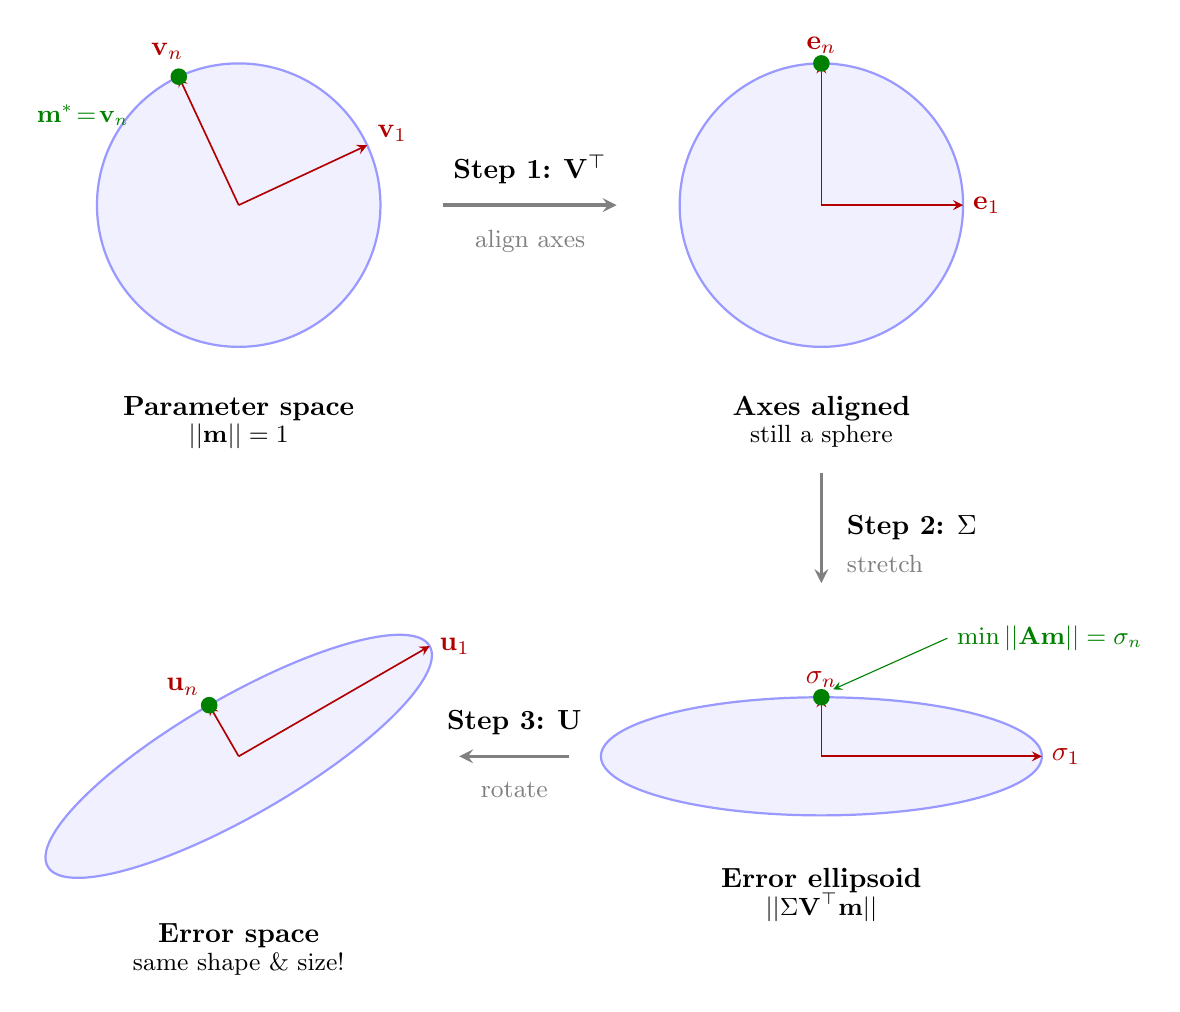
\begin{tikzpicture}[>=stealth, font=\normalsize]

  % ======== TOP ROW ========

  % === Panel 1: Unit sphere in parameter space ===
  \begin{scope}[shift={(0,3.5)}]
    \fill[blue!6] (0,0) circle (1.8);
    \draw[thick, blue!40] (0,0) circle (1.8);
    % V-basis vectors (tilted to show non-axis-aligned)
    \draw[->, semithick, red!70!black] (0,0) -- ({1.8*cos(25)},{1.8*sin(25)});
    \node[red!70!black] at ({2.15*cos(25)},{2.15*sin(25)}) {$\mathbf{v}_1$};
    \draw[->, semithick, red!70!black] (0,0) -- ({1.8*cos(115)},{1.8*sin(115)});
    \node[red!70!black] at ({2.15*cos(115)},{2.15*sin(115)}) {$\mathbf{v}_n$};
    % Green dot: optimal m at v_n
    \fill[green!50!black] ({1.8*cos(115)},{1.8*sin(115)}) circle (3pt);
    \node[green!50!black, left, font=\small] at ({1.5*cos(148)},{1.5*sin(148)+0.35}) {$\mathbf{m}^*\!=\!\mathbf{v}_n$};
    % Subtitle
    \node[below, font=\normalsize\bfseries, align=center] at (0,-2.3) {Parameter space\\[-2pt]{\normalfont\small $||\mathbf{m}||=1$}};
  \end{scope}

  % === Arrow: V^T (horizontal, top row) ===
  \draw[->, very thick, black!50] (2.6, 3.5) -- (4.8, 3.5);
  \node[above] at (3.7, 3.65) {\textbf{Step 1:} $\mathbf{V}^\top$};
  \node[below, font=\small, gray] at (3.7, 3.3) {align axes};

  % === Panel 2: Aligned unit sphere ===
  \begin{scope}[shift={(7.4,3.5)}]
    \fill[blue!6] (0,0) circle (1.8);
    \draw[thick, blue!40] (0,0) circle (1.8);
    \draw[->, semithick, red!70!black] (0,0) -- (1.8,0) node[right] {$\mathbf{e}_1$};
    \draw[->, semithick, red!70!black] (0,0) -- (0,1.8) node[above] {$\mathbf{e}_n$};
    \fill[green!50!black] (0,1.8) circle (3pt);
    \node[below, font=\normalsize\bfseries, align=center] at (0,-2.3) {Axes aligned\\[-2pt]{\normalfont\small still a sphere}};
  \end{scope}

  % === Arrow: Sigma (vertical, right side) ===
  \draw[->, very thick, black!50] (7.4, 0.1) -- (7.4, -1.3);
  \node[right, align=left] at (7.6, -0.6) {\textbf{Step 2:} $\boldsymbol{\Sigma}$};
  \node[right, font=\small, gray] at (7.6, -1.05) {stretch};

  % ======== BOTTOM ROW (right-to-left for clockwise flow) ========

  % === Panel 3: Error ellipsoid (bottom-right, under Panel 2) ===
  \begin{scope}[shift={(7.4,-3.5)}]
    \fill[blue!6] (0,0) ellipse (2.8 and 0.75);
    \draw[thick, blue!40] (0,0) ellipse (2.8 and 0.75);
    \draw[->, semithick, red!70!black] (0,0) -- (2.8,0) node[right] {$\sigma_1$};
    \draw[->, semithick, red!70!black] (0,0) -- (0,0.75) node[above] {$\sigma_n$};
    \fill[green!50!black] (0,0.75) circle (3pt);
    % Annotation arrow
    \draw[->, thin, green!50!black] (1.6, 1.5) -- (0.15, 0.85);
    \node[green!50!black, right, font=\small] at (1.6, 1.5) {$\min ||\mathbf{A}\mathbf{m}|| = \sigma_n$};
    \node[below, font=\normalsize\bfseries, align=center] at (0,-1.3) {Error ellipsoid\\[-2pt]{\normalfont\small $||\boldsymbol{\Sigma}\mathbf{V}^\top\mathbf{m}||$}};
  \end{scope}

  % === Arrow: U (horizontal, bottom row, right-to-left) ===
  \draw[->, very thick, black!50] (4.2, -3.5) -- (2.8, -3.5);
  \node[above] at (3.5, -3.35) {\textbf{Step 3:} $\mathbf{U}$};
  \node[below, font=\small, gray] at (3.5, -3.7) {rotate};

  % === Panel 4: Rotated ellipsoid in error space (bottom-left) ===
  \begin{scope}[shift={(0,-3.5)}]
    \fill[blue!6, rotate=30] (0,0) ellipse (2.8 and 0.75);
    \draw[thick, blue!40, rotate=30] (0,0) ellipse (2.8 and 0.75);
    \draw[->, semithick, red!70!black] (0,0) -- ({2.8*cos(30)},{2.8*sin(30)}) node[right] {$\mathbf{u}_1$};
    \draw[->, semithick, red!70!black] (0,0) -- ({0.75*cos(120)},{0.75*sin(120)}) node[above left] {$\mathbf{u}_n$};
    \fill[green!50!black] ({0.75*cos(120)},{0.75*sin(120)}) circle (3pt);
    \node[below, font=\normalsize\bfseries, align=center] at (0,-2.0) {Error space\\[-2pt]{\normalfont\small same shape \& size!}};
  \end{scope}

\end{tikzpicture}%
}
\end{center}